%%%%%%%%%%%%%%%%%%%%%%%%%%%%%%%%%%%%%%%%%%%%%%%%%%%%%%%%%%%%%%%%%%%%%%%%%%%%%%%%%%
\begin{frame}[fragile]\frametitle{}
\begin{center}
{\Large Decision Tree  - UCI Adults}

{\tiny (Ref: mlcourse.ai Demo 3 – Open Machine Learning Course) }

\end{center}

\end{frame}

%%%%%%%%%%%%%%%%%%%%%%%%%%%%%%%%%%%%%%%%%%%%%%%%%%%%%%%%%%
\begin{frame}[fragile]\frametitle{Problem Info}	
\begin{itemize}
\item Problem: Classify people using demographical data - whether they earn more than \$50,000 per year or not.
\item Dataset location: http://archive.ics.uci.edu/ml/machine-learning-databases/adult
\end{itemize}
\end{frame}

%%%%%%%%%%%%%%%%%%%%%%%%%%%%%%%%%%%%%%%%%%%%%%%%%%%%%%%%%%
\begin{frame}[fragile]\frametitle{Feature Descriptions}	
\begin{itemize}
\item Age – continuous feature
\item Workclass – continuous feature
\item fnlwgt – final weight of object, continuous feature
\item Education – categorical feature
\item Education\_Num – number of years of education, continuous
\item Martial\_Status – categorical feature
\item Occupation – categorical feature
\item Relationship – categorical feature
\item Race – categorical feature
\item Sex – categorical feature
\item Capital\_Gain – continuous feature
\item Capital\_Loss – continuous feature
\item Hours\_per\_week – continuous feature
\item Country – categorical feature
\item Target – earnings level, categorical (binary) feature.
\end{itemize}
\end{frame}

%%%%%%%%%%%%%%%%%%%%%%%%%%%%%%%%%%%%%%%%%%%%%%%%%%%%%%%%%%
\begin{frame}[fragile]\frametitle{Reading train data}	
\begin{lstlisting}
data_train = pd.read_csv('data/adult_train.csv', sep=',')
data_train.tail()
\end{lstlisting}
\begin{center}
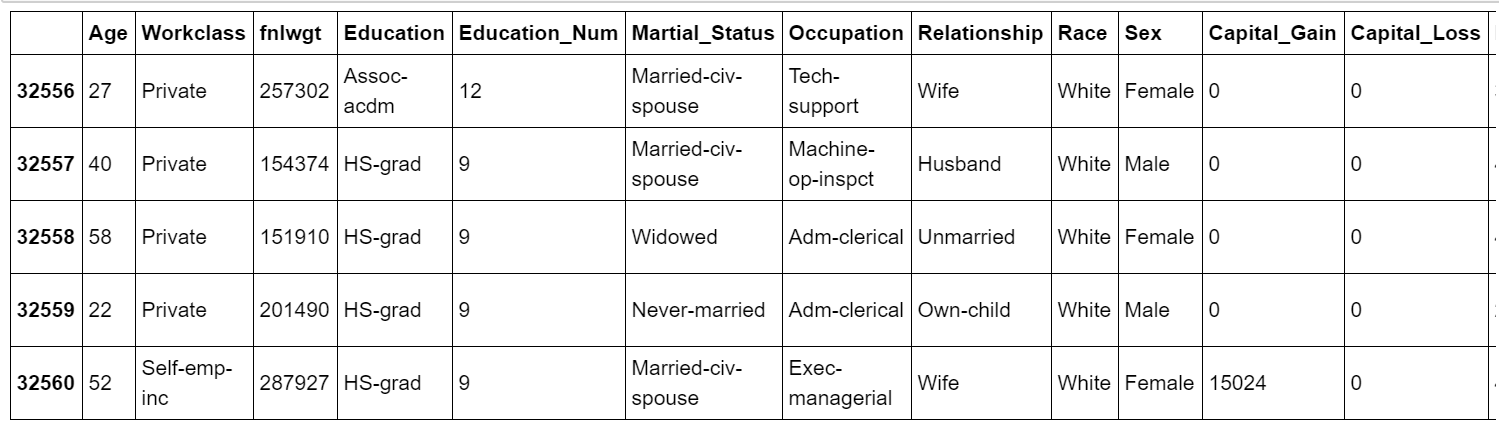
\includegraphics[width=\linewidth,keepaspectratio]{mlcourse14}
\end{center}
\end{frame}

%%%%%%%%%%%%%%%%%%%%%%%%%%%%%%%%%%%%%%%%%%%%%%%%%%%%%%%%%%
\begin{frame}[fragile]\frametitle{Reading test data}	
\begin{lstlisting}
data_test = pd.read_csv('data/adult_test.csv', sep=',')
data_test.tail()
\end{lstlisting}
\begin{center}
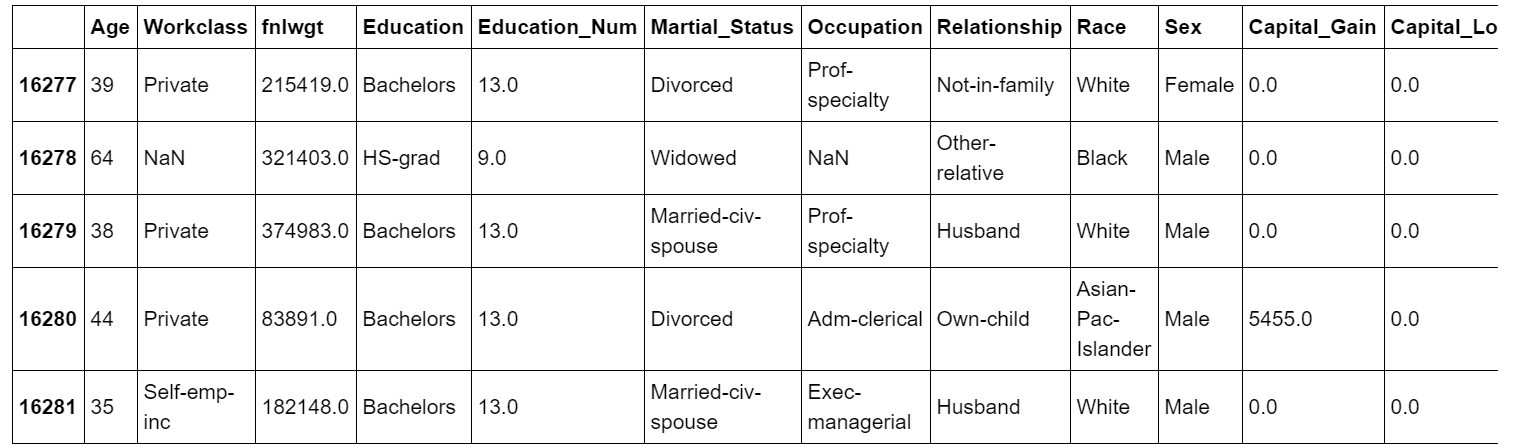
\includegraphics[width=\linewidth,keepaspectratio]{mlcourse15}
\end{center}
\end{frame}

%%%%%%%%%%%%%%%%%%%%%%%%%%%%%%%%%%%%%%%%%%%%%%%%%%%%%%%%%%
\begin{frame}[fragile]\frametitle{Clean test data}	
\begin{lstlisting}
# necessary to remove rows with incorrect labels in test dataset
data_test = data_test[(data_test['Target'] == ' >50K.') | (data_test['Target']==' <=50K.')]

# encode target variable as integer
data_train.loc[data_train['Target']==' <=50K', 'Target'] = 0
data_train.loc[data_train['Target']==' >50K', 'Target'] = 1

data_test.loc[data_test['Target']==' <=50K.', 'Target'] = 0
data_test.loc[data_test['Target']==' >50K.', 'Target'] = 1
\end{lstlisting}
\end{frame}

%%%%%%%%%%%%%%%%%%%%%%%%%%%%%%%%%%%%%%%%%%%%%%%%%%%%%%%%%%
\begin{frame}[fragile]\frametitle{Primary data analysis}	
\begin{lstlisting}
data_test.describe(include='all').T
\end{lstlisting}
\begin{center}
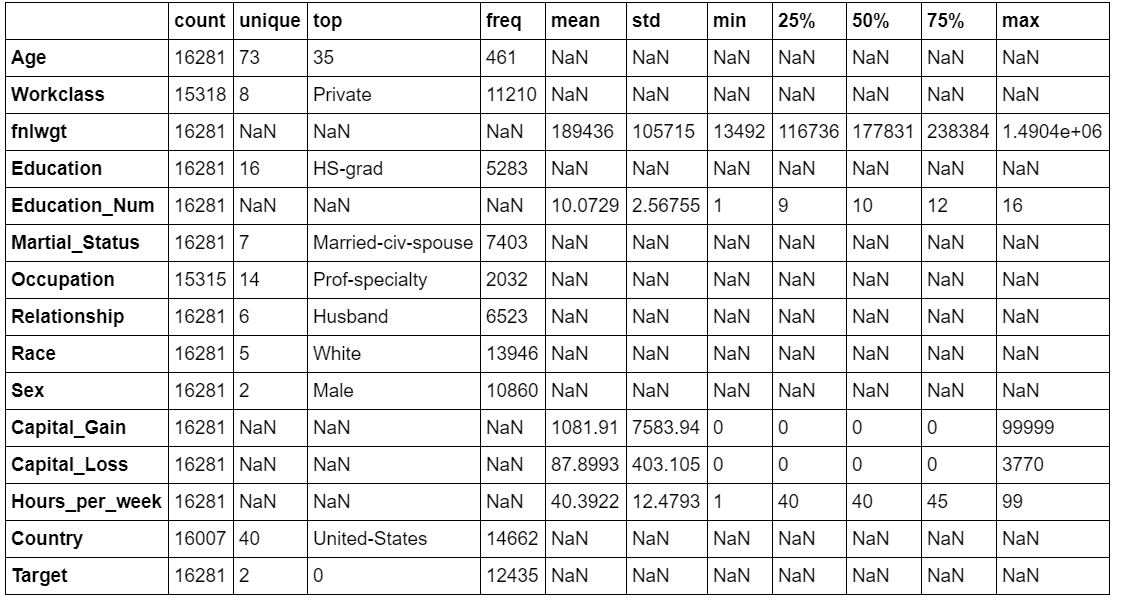
\includegraphics[width=0.7\linewidth,keepaspectratio]{mlcourse16}
\end{center}
\end{frame}

%%%%%%%%%%%%%%%%%%%%%%%%%%%%%%%%%%%%%%%%%%%%%%%%%%%%%%%%%%
\begin{frame}[fragile]\frametitle{Is Target Balanced?}	
\begin{lstlisting}
data_train['Target'].value_counts()

>>
0    24720
1     7841
Name: Target, dtype: int64
\end{lstlisting}
Not at all. Will need measures like F1 score to assess.
\end{frame}

%%%%%%%%%%%%%%%%%%%%%%%%%%%%%%%%%%%%%%%%%%%%%%%%%%%%%%%%%%
\begin{frame}[fragile]\frametitle{Pairwise Plots}	
\begin{lstlisting}
fig = plt.figure(figsize=(25, 15))
cols = 5
rows = np.ceil(float(data_train.shape[1]) / cols)
for i, column in enumerate(data_train.columns):
    ax = fig.add_subplot(rows, cols, i + 1)
    ax.set_title(column)
    if data_train.dtypes[column] == np.object:
        data_train[column].value_counts().plot(kind="bar", axes=ax)
    else:
        data_train[column].hist(axes=ax)
        plt.xticks(rotation="vertical")
plt.subplots_adjust(hspace=0.7, wspace=0.2)
\end{lstlisting}
\end{frame}

%%%%%%%%%%%%%%%%%%%%%%%%%%%%%%%%%%%%%%%%%%%%%%%%%%%%%%%%%%
\begin{frame}[fragile]\frametitle{Pairwise Plots}	
\begin{center}
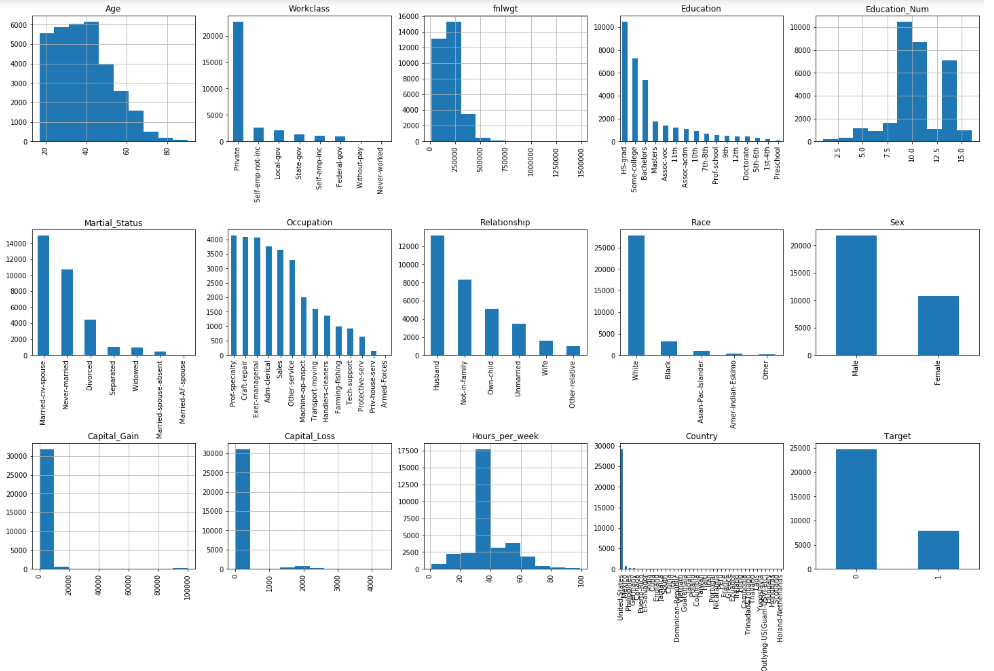
\includegraphics[width=0.8\linewidth,keepaspectratio]{mlcourse17}
\end{center}
\end{frame}

%%%%%%%%%%%%%%%%%%%%%%%%%%%%%%%%%%%%%%%%%%%%%%%%%%%%%%%%%%
\begin{frame}[fragile]\frametitle{Checking data types: Training}	
\begin{lstlisting}
data_train.dtypes

>>
Age                int64
Workclass         object
fnlwgt             int64
Education         object
Education_Num      int64
Martial_Status    object
Occupation        object
Relationship      object
Race              object
Sex               object
Capital_Gain       int64
Capital_Loss       int64
Hours_per_week     int64
Country           object
Target            object
dtype: object
\end{lstlisting}
\end{frame}

%%%%%%%%%%%%%%%%%%%%%%%%%%%%%%%%%%%%%%%%%%%%%%%%%%%%%%%%%%
\begin{frame}[fragile]\frametitle{Checking data types: Testing}	
\begin{lstlisting}
data_test.dtypes

>>
Age                object
Workclass          object
fnlwgt            float64
Education          object
Education_Num     float64
Martial_Status     object
Occupation         object
Relationship       object
Race               object
Sex                object
Capital_Gain      float64
Capital_Loss      float64
Hours_per_week    float64
Country            object
Target             object
dtype: object
\end{lstlisting}
In the test data, age is treated as type object. We need to fix this.
\begin{lstlisting}
data_test['Age'] = data_test['Age'].astype(int)
\end{lstlisting}
\end{frame}

%%%%%%%%%%%%%%%%%%%%%%%%%%%%%%%%%%%%%%%%%%%%%%%%%%%%%%%%%%
\begin{frame}[fragile]\frametitle{Checking data types: Testing}	
Cast all float features to int type to keep types consistent between our train and test data.
\begin{lstlisting}
data_test['fnlwgt'] = data_test['fnlwgt'].astype(int)
data_test['Education_Num'] = data_test['Education_Num'].astype(int)
data_test['Capital_Gain'] = data_test['Capital_Gain'].astype(int)
data_test['Capital_Loss'] = data_test['Capital_Loss'].astype(int)
data_test['Hours_per_week'] = data_test['Hours_per_week'].astype(int)
\end{lstlisting}
\end{frame}

%%%%%%%%%%%%%%%%%%%%%%%%%%%%%%%%%%%%%%%%%%%%%%%%%%%%%%%%%%
\begin{frame}[fragile]\frametitle{Missing Data}	
Fill in missing data for continuous features with their median values, for categorical features with their mode.

\begin{lstlisting}
categorical_columns = [c for c in data_train.columns 
                       if data_train[c].dtype.name == 'object']
numerical_columns = [c for c in data_train.columns 
                     if data_train[c].dtype.name != 'object']

>>
categorical_columns: ['Workclass', 'Education', 'Martial_Status', 'Occupation', 'Relationship', 'Race', 'Sex', 'Country', 'Target']
numerical_columns: ['Age', 'fnlwgt', 'Education_Num', 'Capital_Gain', 'Capital_Loss', 'Hours_per_week']

for c in categorical_columns:
    data_train[c].fillna(data_train[c].mode(), inplace=True)
    data_test[c].fillna(data_train[c].mode(), inplace=True)
    
for c in numerical_columns:
    data_train[c].fillna(data_train[c].median(), inplace=True)
    data_test[c].fillna(data_train[c].median(), inplace=True)

\end{lstlisting}
\end{frame}

%%%%%%%%%%%%%%%%%%%%%%%%%%%%%%%%%%%%%%%%%%%%%%%%%%%%%%%%%%
\begin{frame}[fragile]\frametitle{Make Data Numerical}	
We'll dummy code some categorical features: Workclass, Education, Martial\_Status, Occupation, Relationship, Race, Sex, Country. 
It can be done via pandas method get\_dummies
\begin{lstlisting}
data_train = pd.concat([data_train[numerical_columns],
    pd.get_dummies(data_train[categorical_columns])], axis=1)

data_test = pd.concat([data_test[numerical_columns],
    pd.get_dummies(data_test[categorical_columns])], axis=1)
\end{lstlisting}
\end{frame}

%%%%%%%%%%%%%%%%%%%%%%%%%%%%%%%%%%%%%%%%%%%%%%%%%%%%%%%%%%
\begin{frame}[fragile]\frametitle{Any Diff between Train and Test?}	
\begin{lstlisting}
set(data_train.columns) - set(data_test.columns)
>>
{'Country_ Holand-Netherlands'}

data_train.shape, data_test.shape
((32561, 106), (16281, 105))

data_test['Country_ Holand-Netherlands'] = 0
\end{lstlisting}
There is no Holland in the test data. Create new zero-valued feature.
\end{frame}

%%%%%%%%%%%%%%%%%%%%%%%%%%%%%%%%%%%%%%%%%%%%%%%%%%%%%%%%%%
\begin{frame}[fragile]\frametitle{Prepare Data}	
\begin{lstlisting}
categorical_columns = [c for c in data_train.columns 
X_train = data_train.drop(['Target'], axis=1)
y_train = data_train['Target']

X_test = data_test.drop(['Target'], axis=1)
y_test = data_test['Target']
\end{lstlisting}
\end{frame}

%%%%%%%%%%%%%%%%%%%%%%%%%%%%%%%%%%%%%%%%%%%%%%%%%%%%%%%%%%
\begin{frame}[fragile]\frametitle{Decision tree without parameter tuning}	
Train a decision tree (DecisionTreeClassifier) with a maximum depth of 3, and evaluate the accuracy metric on the test data. Use parameter random\_state = 17 for results reproducibility.
\begin{lstlisting}
tree = DecisionTreeClassifier(max_depth=3, random_state=17)
tree.fit(X_train, y_train)

>>
DecisionTreeClassifier(class_weight=None, criterion='gini', max_depth=3,
            max_features=None, max_leaf_nodes=None,
            min_impurity_decrease=0.0, min_impurity_split=None,
            min_samples_leaf=1, min_samples_split=2,
            min_weight_fraction_leaf=0.0, presort=False, random_state=17,
            splitter='best')
\end{lstlisting}
\end{frame}

%%%%%%%%%%%%%%%%%%%%%%%%%%%%%%%%%%%%%%%%%%%%%%%%%%%%%%%%%%
\begin{frame}[fragile]\frametitle{Predictions}	
Make a prediction with the trained model on the test data.
\begin{lstlisting}
tree_predictions = tree.predict(X_test) 
accuracy_score(y_test,tree_predictions)
>>
0.8447884036607088
\end{lstlisting}
\end{frame}


%%%%%%%%%%%%%%%%%%%%%%%%%%%%%%%%%%%%%%%%%%%%%%%%%%%%%%%%%%
\begin{frame}[fragile]\frametitle{Decision tree with parameter tuning}	
Train a decision tree (DecisionTreeClassifier, random\_state = 17). Find the optimal maximum depth using 5-fold cross-validation (GridSearchCV).
\begin{lstlisting}
tree_params = {'max_depth': range(2, 11)}
locally_best_tree = GridSearchCV(DecisionTreeClassifier(random_state=17),tree_params, cv=5)                  
locally_best_tree.fit(X_train, y_train)

print("Best params:", locally_best_tree.best_params_)
print("Best cross validaton score", locally_best_tree.best_score_)
>>
Best params: {'max_depth': 9}
Best cross validaton score 0.8562697705844415
\end{lstlisting}
\end{frame}

%%%%%%%%%%%%%%%%%%%%%%%%%%%%%%%%%%%%%%%%%%%%%%%%%%%%%%%%%%
\begin{frame}[fragile]\frametitle{Train}	
Train a decision tree with maximum depth of 9 (it is the best max\_depth in my case), and compute the test set accuracy. Use parameter random\_state = 17 for reproducibility.
\begin{lstlisting}
tuned_tree = DecisionTreeClassifier(max_depth=9, random_state=17)
tuned_tree.fit(X_train, y_train)
tuned_tree_predictions = tuned_tree.predict(X_test)
accuracy_score(y_test, tuned_tree_predictions)

>>
0.8471838339168356
\end{lstlisting}
\end{frame}


%%%%%%%%%%%%%%%%%%%%%%%%%%%%%%%%%%%%%%%%%%%%%%%%%%%%%%%%%%
\begin{frame}[fragile]\frametitle{Random forest without parameter tuning}	
Train a random forest (RandomForestClassifier). Set the number of trees to 100 and use random\_state = 17.
\begin{lstlisting}
rf = RandomForestClassifier(n_estimators=100, random_state=17)
rf.fit(X_train, y_train)

>>
RandomForestClassifier(bootstrap=True, class_weight=None, criterion='gini',
            max_depth=None, max_features='auto', max_leaf_nodes=None,
            min_impurity_decrease=0.0, min_impurity_split=None,
            min_samples_leaf=1, min_samples_split=2,
            min_weight_fraction_leaf=0.0, n_estimators=100, n_jobs=1,
            oob_score=False, random_state=17, verbose=0, warm_start=False)
\end{lstlisting}
\end{frame}

%%%%%%%%%%%%%%%%%%%%%%%%%%%%%%%%%%%%%%%%%%%%%%%%%%%%%%%%%%
\begin{frame}[fragile]\frametitle{Score}	
\begin{lstlisting}
cv_scores = cross_val_score(rf, X_train, y_train, cv=3)
cv_scores, cv_scores.mean()

>>
(array([0.85203612, 0.85553713, 0.85930158]), 0.8556249401626314)
\end{lstlisting}
\end{frame}

%%%%%%%%%%%%%%%%%%%%%%%%%%%%%%%%%%%%%%%%%%%%%%%%%%%%%%%%%%
\begin{frame}[fragile]\frametitle{Predictions}	
Make predictions for the test data and assess accuracy.
\begin{lstlisting}
forest_predictions = rf.predict(X_test) 
accuracy_score(y_test,forest_predictions)

>>
0.8576254529820035
\end{lstlisting}
\end{frame}

%%%%%%%%%%%%%%%%%%%%%%%%%%%%%%%%%%%%%%%%%%%%%%%%%%%%%%%%%%
\begin{frame}[fragile]\frametitle{Random forest with parameter tuning}	
Train a random forest (RandomForestClassifier). Tune the maximum depth and maximum number of features for each tree using GridSearchCV.
\begin{lstlisting}
forest_params = {'max_depth': range(10, 16),
                 'max_features': range(5, 105, 20)}
locally_best_forest = GridSearchCV(RandomForestClassifier(n_estimators=10, 
				random_state=17,n_jobs=-1),forest_params, cv=3, verbose=1)
locally_best_forest.fit(X_train, y_train)
print("Best params:", locally_best_forest.best_params_)
print("Best cross validaton score", locally_best_forest.best_score_)
>>
Best params: {'max_depth': 11, 'max_features': 25}
Best cross validaton score 0.8618285679186757
\end{lstlisting}
\end{frame}

%%%%%%%%%%%%%%%%%%%%%%%%%%%%%%%%%%%%%%%%%%%%%%%%%%%%%%%%%%
\begin{frame}[fragile]\frametitle{Predictions}	
Make predictions for the test data and assess accuracy.
\begin{lstlisting}
tuned_forest_predictions = locally_best_forest.predict(X_test) 
accuracy_score(y_test,tuned_forest_predictions)

>>
0.862600577360113
\end{lstlisting}
\end{frame}